All test results contained in this \thesis{} were performed on one of two
servers with the following specifications. The following specifications were
obtained using the \software{Hardware Lister}[lshw] tool.

%%%%%%%%%%%%%%%%%%%%%%%%%%%%%%%%%%%%%%%%%%%%%%%%%%%%%%%%%%%%%%%%%%%%%%%%%%%%%%%%
% HOSTNAME: tuna
%%%%%%%%%%%%%%%%%%%%%%%%%%%%%%%%%%%%%%%%%%%%%%%%%%%%%%%%%%%%%%%%%%%%%%%%%%%%%%%%
\section{Host name: tuna}
\label{specs:tuna}
The specifications for the \hostname{tuna} are detailed below.

% Hardware Specifications
\subsection{Hardware Specifications}
\label{specs:tuna:hardware}
\begin{specifications}
    \specificationGroup{\gls{CPU}}
        \specification{Product}{\IntelXeon{} \glsname{CPU} E5506 @ 2.13GHz}
        \specification{Size}{2133 MHz}
        \specification{Capacity}{3600 MHz}
        \specification{Width}{64 bits}
        \specification{Clock}{505 MHz}
        \specification{Cores}{4}
        \specification{L1 cache}{128 KiB (internal write-back data)}
        \specification{L2 cache}{1 MiB (internal write-back unified)}
        \specification{L3 cache}{4 MiB (internal write-back unified)}
        \specification{CPU capabilities}{
            x86-64, fpu, fpu\_exception, wp, vme, de, pse, tsc, msr, pae, mce,
            cx8, apic, sep, mtrr, pge, mca, cmov, pat, pse36, clflush, dts,
            acpi, mmx, fxsr, sse, sse2, ss, ht, tm, pbe, syscall, nx, rdtscp,
            constant\_tsc, arch\_perfmon, pebs, bts, rep\_good, nopl, xtopology,
            nonstop\_tsc, aperfmperf, pni, dtes64, monitor, ds\_cpl, vmx, est,
            tm2, ssse3, cx16, xtpr, pdcm, dca, sse4\_1, sse4\_2, popcnt,
            lahf\_lm, tpr\_shadow, vnmi, flexpriority, ept, vpid.}
    \endspecificationGroup

    \specificationGroup{Memory}
        \specification{Description}{\glsname{DIMM} \glsname{DDR}3 Synchronous 1333 MHz}
        \specification{Size}{8 GiB}
        \specification{Width}{64 bits}
        \specification{Clock}{1333 MHz}
    \endspecificationGroup
\end{specifications}

% Software Specifications
\subsection{Software Specifications}
\label{specs:tuna:software}
\begin{specifications}
    \specification{gcc}{gcc (Ubuntu/Linaro 4.6.1-9ubuntu3) 4.6.1}
    \specification{ld}{\glsname{GNU} ld (\glsname{GNU} Binutils for Ubuntu) 2.21.53.20110810}
    \specification{MATLAB}{MATLAB 7.13.0.564 (R2011b)}
\end{specifications}

% Operating System Specifications
\subsection{Operating System Specifications}
\label{specs:tuna:os}
\begin{specifications}
    \specification{Operating System}{Ubuntu 11.10}
    \specification{Platform}{x86\_64}
    \specification{Kernel version}{3.0.0-17-generic}
\end{specifications}

%%%%%%%%%%%%%%%%%%%%%%%%%%%%%%%%%%%%%%%%%%%%%%%%%%%%%%%%%%%%%%%%%%%%%%%%%%%%%%%%
% HOSTNAME: ubuntu-vm
%%%%%%%%%%%%%%%%%%%%%%%%%%%%%%%%%%%%%%%%%%%%%%%%%%%%%%%%%%%%%%%%%%%%%%%%%%%%%%%%
\section{Host name: ubuntu-vm}
\label{specs:ubuntu-vm}
The specifications for the \hostname{ubuntu-vm} are detailed below.

% Hardware Specifications
\subsection{Hardware Specifications}
\label{specs:ubuntu-vm:hardware}
\begin{specifications}
    \specificationGroup{CPU}
        \specification{Product}{\IntelCoreiSeven{} \glsname{CPU} 950 @ 3.07GHz}
        \specification{Size}{3067 MHz}
        \specification{Capacity}{4230 MHz}
        \specification{Width}{64 bits}
        \specification{Cores}{8}
        \specification{L1 cache}{16 KiB (asynchronous internal write-back)}
        \specification{L2 cache}{256 KiB (burst external write-back)}
        \specification{CPU Capabilities}{
            fpu, fpu\_exception, wp, vme, de, pse, tsc, msr, pae, mce, cx, apic,
            sep, mtrr, pge, mca, cmov, pat, pse36, clflush, dts, acpi, mmx,
            fxsr, sse, sse2, ss, ht, syscall, nx, rdtscp, x86-64, constant\_tsc,
            arch\_perfmon, pebs, bts, nopl, xtopology, tsc\_reliable,
            nonstop\_tsc, aperfmperf, pni, ssse3, cx16, sse4\_1, sse4\_2,
            popcnt, hypervisor, lahf\_lm, ida, dtherm.}
    \endspecificationGroup

    \specificationGroup{Memory}
        \specification{Description}{\glsname{DIMM} \glsname{DRAM} EDO}
        \specification{Size}{16 GiB}
        \specification{Width}{32 bits}
    \endspecificationGroup
\end{specifications}

% Software Specifications
\subsection{Software Specifications}
\label{specs:ubuntu-vm:software}
\begin{specifications}
    \specification{gcc}{gcc (Ubuntu/Linaro 4.6.1-9ubuntu3) 4.6.1}
    \specification{ld}{\glsname{GNU} ld (\glsname{GNU} Binutils for Ubuntu) 2.22}
    \specification{MATLAB}{MATLAB 7.14.0.739 (R2012a)}
\end{specifications}

% Operating System Specifications
\subsection{Operating System Specifications}
\label{specs:ubuntu-vm:os}
\begin{specifications}
    \specification{Operating System}{Ubuntu 12.04}
    \specification{Platform}{x86\_64}
    \specification{Kernel version}{3.2.0-29-generic}
\end{specifications}

%%%%%%%%%%%%%%%%%%%%%%%%%%%%%%%%%%%%%%%%%%%%%%%%%%%%%%%%%%%%%%%%%%%%%%%%%%%%%%%%
% FPGA
%%%%%%%%%%%%%%%%%%%%%%%%%%%%%%%%%%%%%%%%%%%%%%%%%%%%%%%%%%%%%%%%%%%%%%%%%%%%%%%%
\section{FPGA}
\label{specs:fpga}
\label{zynq}

% Introduction
\subsection{Introduction}
\label{specs:fpga:introduction}
\label{zynq:introduction}
\nocite{Zynq7000:ProductBrief,Zynq7000:UserGuide}
In this \thesis{}, the \gls{FPGA} that was used was a \Xilinx{} Z7020CLG484-1
from the ``Zynq-7000'' product series. This device has an \ARM{} dual-core
\Cortex{}-A9 processor, as well as \Xilinx{} 28nm programmable logic. An image
of a \Xilinx{} Zynq-7000 series device is shown in \autoref{fig:zynq:zc702}.

\begin{figure}
    \centering
    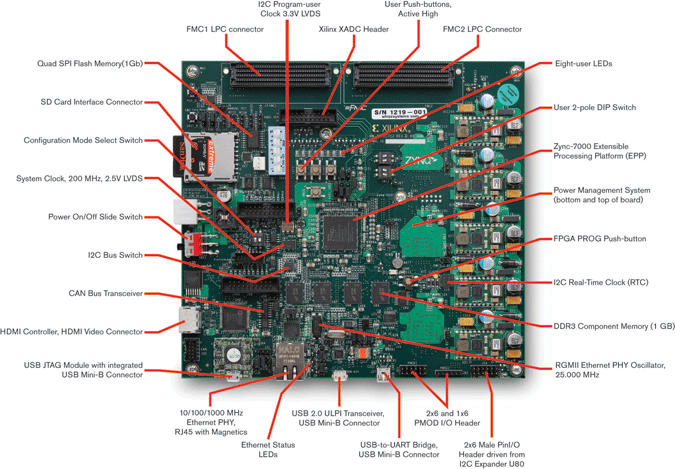
\includegraphics[width=0.5\textwidth]{xilinx/zc702-base-board}
    \caption{A Xilinx ZC7020 \gls{FPGA}}
    \label{fig:zynq:zc702}
\end{figure}

% Board Features
\subsection{Board Features}
\label{specs:fpga:features}
\label{zynq:features}
\nocite{Zynq7000:UserGuide}
\begin{itemize}
    \item Zynq-7000 XC7Z020-1CLG484C \gls{EPP}
    \item 1 GB \gls{DDR}3 component memory (four 256 Mb $\times 8$ devices)
    \item 128 Mb Quad \gls{SPI} flash memory
    \item \gls{USB} 2.0 ULPI (UTMI+ low pin interface) transceiver
    \item \gls{SD} connector
    \item \gls{USB} \gls{JTAG} interface via Digilent module
    \item Clock sources:
    \begin{itemize}
        \item Fixed 200 MHz \gls{LVDS} oscillator (differential)
        \item \gls{I2C} programmable \gls{LVDS} oscillator (differential)
        \item Fixed 33.33 MHz \gls{LVCMOS} oscillator (single-ended)
    \end{itemize}
    \item Ethernet \gls{PHY} \gls{RGMII} interface with RJ-45 connector
    \item \gls{USB}-to-\gls{UART} bridge
    \item \gls{HDMI} codec
    \item \gls{I2C} bus

    \item \gls{I2C} bus multiplexed to:
    \begin{itemize}
        \item Si570 user clock
        \item ADV7511 \gls{HDMI} codec
        \item M24C08 \gls{EEPROM} (1 kB)
        \item 1-To-16 TCA6416APWR port expander
        \item RTC-8564JE real time clock
        \item FMC1 LPC connector
        \item FMC2 LPC connector
        \item \gls{PMBUS} data/clock
    \end{itemize}
    \item Status \glspl{LED}:
    \begin{itemize}
        \item Ethernet status
        \item Power good
        \item \gls{FPGA} INIT
        \item \gls{FPGA} DONE
    \end{itemize}
    \item User \gls{IO}:
    \begin{itemize}
        \item Eight user \glspl{LED}
        \item Two \gls{PL} user push buttons
        \item \gls{PL} user \gls{DIP} switch (2-pole)
        \item Two \gls{PS} push buttons shared with \gls{PS} 2-pole \gls{DIP}
            switch
        \item Two \gls{PS} user \glspl{LED}
        \item Dual row Pmod \gls{GPIO} header
        \item Single row Pmod \gls{GPIO} header
    \end{itemize}
    \item \gls{EPP} \gls{PS} Reset Push buttons:
    \begin{itemize}
        \item SRST\_B \gls{PS} reset button
        \item POR\_B \gls{PS} reset button
    \end{itemize}
    \item Two VITA 57.1 FMC LPC connectors
    \item Power on/off slide switch
    \item Power management with \gls{PMBUS} voltage and current monitoring via
        TI power controllers
    \item Dual 12-bit 1 MSPS XADC analog-to-digital front end

    \item Configuration options:
    \begin{itemize}
        \item Quad \gls{SPI} flash memory
        \item \gls{USB} \gls{JTAG} configuration port (Digilent module)
        \item Platform cable header \gls{JTAG} configuration port
        \item 20-pin \gls{PL} \gls{PJTAG} header
        \item 20-pin \gls{PL} \gls{JTAG} header
    \end{itemize}
\end{itemize}

\begin{figure}
    \centering
    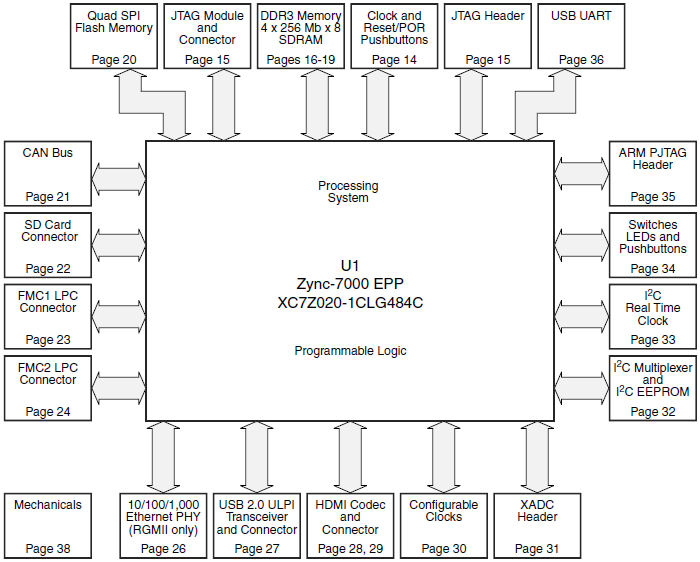
\includegraphics[width=0.5\textwidth]{xilinx/block-diagram}
    \caption{A block diagram for the Xilinx Z7020 series \glspl{FPGA}}
    \label{fig:zynq:blockDiagram}
\end{figure}